\section{Auswertung zum Shinriki-Oszillator}

\subsection{Phasendiagramm}
Im Folgenden wurde ein Phasendiagramm des Shinrinki-Oszillators mit den Werten \(R_1\) und \(R_2\) erstellt. Dafür wurden Schnittpunkte der Phasenübergänge ermittelt und mithilfe eines Python-Skripts wurde diese Punkte mit einer Funktion verbunden. Daraus ergibt sich folgende Abbildung, welche die Übergänge der verschiedenen Phasen abhängig von den Werten der Widerstände darstellen. Jede Line stellt dabei einen Phasenübergang dar.

\begin{figure}[h]
    \centering
    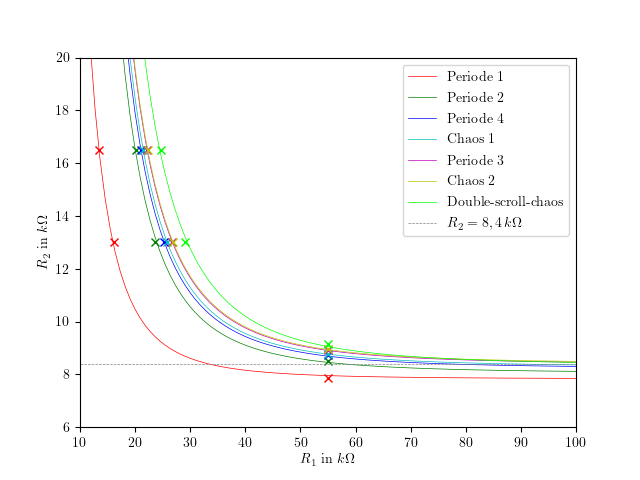
\includegraphics[scale=0.75]{AuswPaul/PhasendiagrammFertig.png}
    \label{fig:Phasendiagramm}
    \caption{Phasendiagramm}
\end{figure}

Die Funktion welche benutzt wurde, um die Punkte zu verbinden ist:
\begin{align}
    f = \frac{a}{x^3} +b
\end{align}

Diese Funktion wurde ausgewählt, indem mehrere verschiedene Funktionen ausprobiert wurden. Nachfolgend ausgewählte Funktionen zum Vergleich, um die Auswahl nachvollziehen zu können.
\begin{figure}[h]

    \centering
    
    \begin{subfigure}[b]{0.45\textwidth}
        \centering
        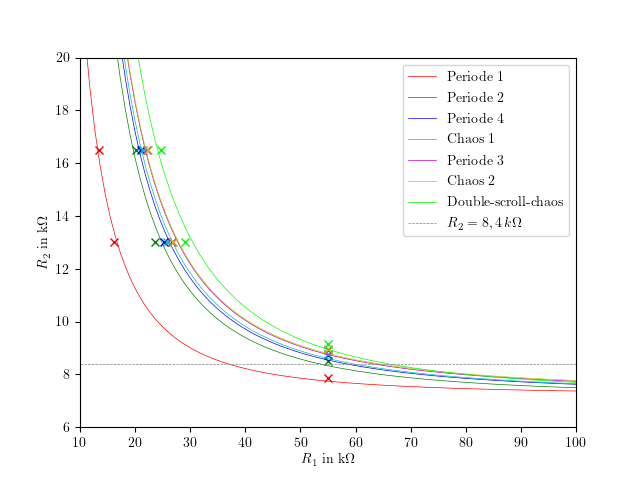
\includegraphics[width=\textwidth]{AuswPaul/PhaDiaGrad-2.png}
        \caption{$f = \frac{a}{x^2} + b$}
    \end{subfigure}
    \hfill
    \begin{subfigure}[b]{0.45\textwidth}
        \centering
        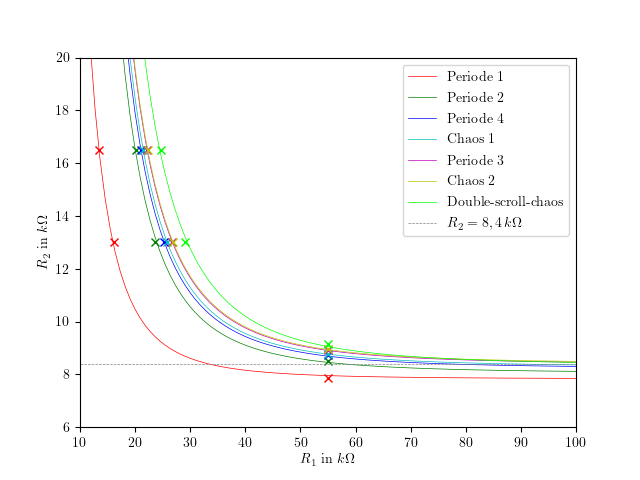
\includegraphics[width=\textwidth]{AuswPaul/PhasendiagrammFertig.png}
        \caption{$f = \frac{a}{x^3} + b$}
    \end{subfigure}
    \\
    \begin{subfigure}[b]{0.45\textwidth}
        \centering
        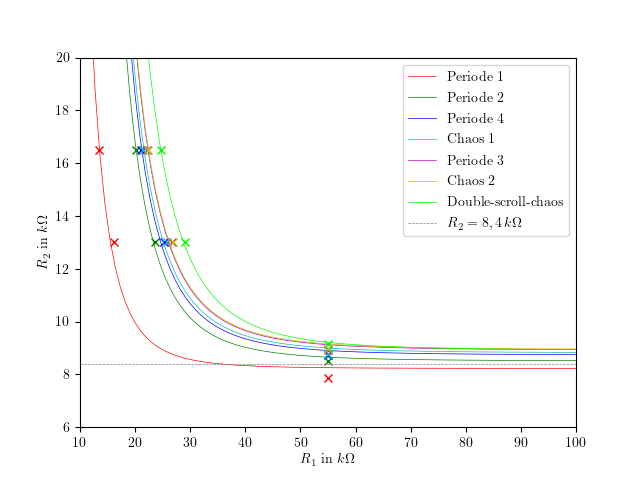
\includegraphics[width=\textwidth]{AuswPaul/PhaDiaGrad-4.png}
        \caption{$f = \frac{a}{x^4} + b$}
    \end{subfigure}
    \caption{Vergleich verschiedener 'Fitting'-Funktionen}
    \label{fig:PhasenDiaVergl}
    \end{figure}

\newpage
\subsection{Schnitt durch das Phasendiagramm}
Nun wird für einen festen Wert (\(R_2 = 8,4 k\Omega\)) ein Schnitt durch das Phasendiagramm erzeugt, indem \(R_1\) variiert wird und die Veränderungen aufmerksam beobachtet werden. \\
Im Folgenden unsere Beobachtungen bei ausgewählten Werten von \(R_1\).

\subsection{Bifurkationsdiagramm}
Um ein Bifurkationsdiagramm zu erstellen würde ähnlich zum Schnitt durch das Phasendiagramm ein fester Wert (\(R_2=8,4k \Omega\)) eingestellt. Unter zuhilfenahme des Labview Messprogramms konnte nun durch Variation von \(R_1\) folgendes Diagramm erstellt werden.



\subsection{Feigenbaum-Konstante}

Um die Feigenbaum-Konstante zu bestimmen wurden die Werde, bein denen eine Periodenverdopplung auftrat, ermittelt. Diese wurden durch eine separate Messung aufgenommen und nicht aus obigen Bifurkationsdiagramm abgelesen. Damit wird versucht genauere werte zu erhalten. Da für das Bifurkationsdiagramm die Messdauer, im Vergleich zum direkten Suchen der Periodenverdopplungen, deutlich größer ist, ist es wahrscheinlicher, dass Störquellen, wie Temperaturveränderungen der Messgeräte, die Werte verfälschen.\\

Die Feigenbaum-Konstante \(\delta\) kann folgendermaßen berechnet werden: 
\begin{align}
    \delta = \lim_{n \to \infty} \delta_n \\
    \delta_n = \frac{r_n - r_{n-1}}{r_{n+1} -r_n}
\end{align}

Der Literaturwert der Feigenbaum-Konstante ist: \(\delta = 4,6692...\)\\

Folgende Werte wurden gemessen: \\
\begin{tabular}{c c c}
    $r_1$ & $r_2$ & $r_3$\\
    \hline
    59 & 65,6 & 67,6
\end{tabular}

Damit ergibt sich ein Feigenbaum-Konstante von \(\delta = (? \pm ?)\)

\subsection{Zum Einbettungstheorem}